%==========================================================
% The OpenCms synchronization
%==========================================================
\chapter{The OpenCms synchronization}
\label{synchronization}

\section{What is synchronization?}
%============================================================================
The synchronization tool \index{synchronization} is used to synchronize \index{synchronize} files in the Virtual File System \index{Virtual File System} of OpenCms and their corresponding files in the Server File System \index{Server File System}.

It's a feature for development only. It speeds up the development cycle because you can modify the file on your Server File System with your favourite application and update the file in the file system of OpenCms.

\index{synchronizationmanagement}
\section{Manage the properties for OpenCms synchronization}
%============================================================================
The synchronization requires some entries in the {\dir
registry.xml}. You will find the registry in your configuration
path of OpenCms ({\dir config/}). You need to enable and modify
the following section:

\begin{xml}
<syncpath>c:/work41/sync</syncpath>\\
<syncproject>\_syncProject</syncproject>\\
<syncresource>\\
\xtaba  <res1>/content/</res1>\\
\xtaba  <res2>/download/</res2>\\
\xtaba  <res3>/pics/</res3>\\
</syncresource>\\
\end{xml}

The {\tag <syncpath>} \index{syncpath} is the path on your server
where you want to save the synchronized files. The {\tag
<syncproject>} \index{syncproject} is the name of your project in
OpenCms whose files you want to synchronize. In the section {\tag
<syncresource>} \index{syncresource} you put the names of the
resources you want to be synchronized. Put each resourcename
between a tag named {\tag <resx></resx>} where the {\name x} is a
serial number.

To make it easier for you to manage these entries there is a
management tool in the backoffice. Only administrators are allowed
to manage the synchronization properties.

\begin{figure}[hbt]

\begin{minipage}[b]{0.499\linewidth}
  \begin{center}
  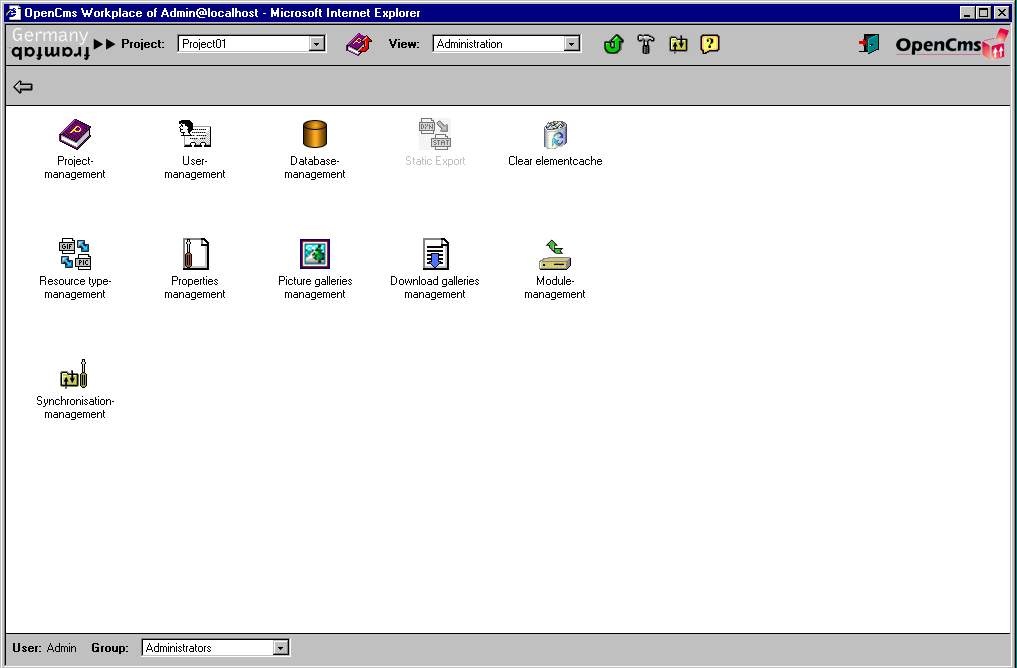
\includegraphics[clip,width=\sgw]
                   {pics/synchronize/syncprop01}
 \end{center}
\end{minipage}
\hfill
\begin{minipage}[b]{0.499\linewidth}
   \begin{center}
   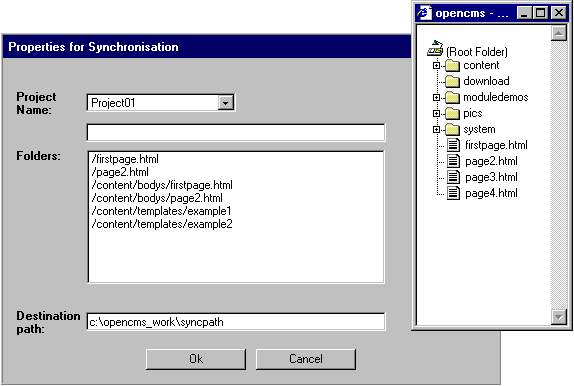
\includegraphics[clip,width=\sgw]
                   {pics/synchronize/syncprop02}
   \end{center}
\end{minipage}
\caption[The synchronization management icon and dialog]
           {The synchronization management icon and dialog}
 \label{syncproperties}

\end{figure}

A click on the icon will open the dialog for synchronization
management. If the entries for synchronization already exist in
the {\dir registry.xml}, they will be shown in the dialog.

You can choose any project from the project list. The list
contains your accessible projects except the online project. So
there must be at least one offline project. When you have chosen a
project the folder tree, that you get with the folder button,
shows the resources in this project. By clicking on a resource you
can add it to the resource list for synchronization. You can also
add resources by filling in the resource name into the field above
the resource list and clicking the arrow button. To remove
resources from the list you use the delete button.

The third entry that is needed is the destination path on your
server.

When you choose all entries you can update the registry by
clicking on 'OK'. There will be errormessages if you left the
project, the resource list or the destination path empty or if a
resource can not be read from the chosen project.

\section{How to synchronize}
%============================================================================

If there are the required entries in the registry.xml the button
for synchronization will appear in the head section between the
icons for the preferences and the help (Figure~\ref{syncicon}).

\begin{figure}[hbt]
\begin{center}
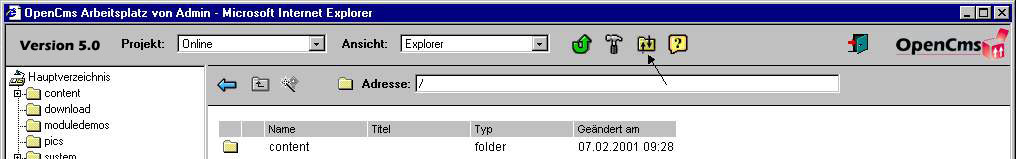
\includegraphics[width=\sgw]
                   {pics/synchronize/syncico}
\caption[The button for synchronization]
           {The button for synchronization}
\label{syncicon}
\end{center}
\end{figure}

A click on the button will start the synchronization. If the project for synchronization, which you specified in the registry, does not exist it will be created and the resources that should be synchronized will be copied from the online project to the synchronization project.

The synchronization will not work if there is more than one project with the name of the synchronization project or if the resource to be synchronized does not exist in the project.

\section{How the files are synchronized}
%============================================================================
First the resource and all its subresources are read from the Virtual File System and checked for changes.

\begin{itemize}
\item The resources that does not exist on the Server File System will be created.
\item If the resource is marked as deleted the corresponding resource will be deleted from the Server File System.
\item Files are compared with the entries in the {\dir synchronize.list}.
\end{itemize}

The {\dir synchronize.list} is created after the synchronization and contains the name of each synchronized file and the date of its last modification in the Virtual File System and the Server File System.

\begin{itemize}
\item If the date of the last modification of the file on the Virtual File System is after the corresponding date in the {\dir synchronize.list} the modification date of the file on the server is checked.
    \begin{itemize}
    \item If the date of the file on the server has not changed after the last synchronization, the file will be updated with the content of the file on the Virtual File System.
    \item Has the file be changed on the Server File System, too, it will be copied to a backupfile (the backupfile is marked with a leading {\name \$}) and updated with the content of the file on the Virtual File System.
    \end{itemize}
\item If the file has not be changed on the Virtual File System but on the Server File System, the file on the Virtual File System will be updated with the content of the file on the Server File System.
\end{itemize}

After the resources on the Virtual File System were checked, the filelist of the resource on the Server File System is read. The Virtual File System is checked if it contains all of the files and folders in this list. Files and folders that does not exist in the Virtual File System are created.

%%% Local Variables:
%%% mode: latex
%%% TeX-master: "OpenCmsDoc"
%%% End:
